\subsection{Modultest af SD kort driver}

SD kort modulet er først testet med Analog Discovery, for at klargøre hvorvidt SPI protokollen sendes korrekt, og derefter gennem debug med påsat skærm- og SD kortmodul.
Under testen er Atmel-ICE med JTAG interface brugt til programmering og debug.\\
Analog Discovery er påsat port b på Atmega2560 og køres gennem Waveforms med Logic Analyzer.
På figur \ref{fig:SPIanalog} ses det at kommandoen, CMD1 fra Part1\_Physical\_Layer\_Simplified\_Specification\_Ver6.00, sendes fra Arduinoen problemfrit og SPI beskeden tolkes af Waveforms. De forekommende Clockcycles uden tilhørende data er for at sikre SD kortets initialisering.
 
\begin{figure}[H]
	\center
	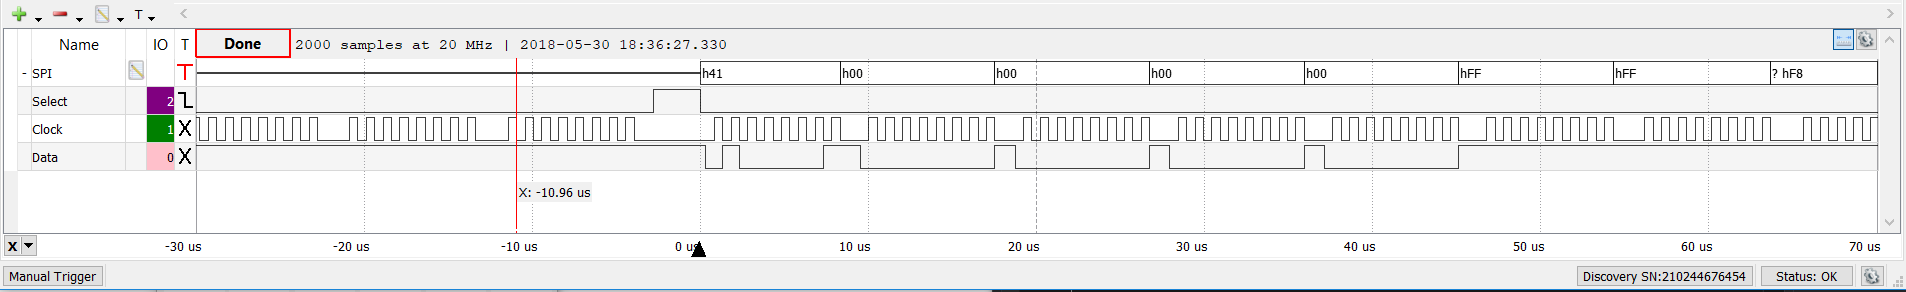
\includegraphics[width=1.0\textwidth]{Figur/SPIoutputSDTest.png}
	\caption{SPI kommando CMD8 fra Arduino Atmega2560}
	\label{fig:SPIanalog}
\end{figure}

Under debugging testes SD Driveren sammen med det tilhørende modul. Problemet med at debugge brugen af SPI kommandoer forekommer da SPI data registret ikke kan aflæses som watch i Atmel Studio, og registret tømmes også under skrivning/læsning til dette. Derfor er der brugt UART til terminalvinduet til at aflæse værdierne.

\begin{figure}[H]
	\center
	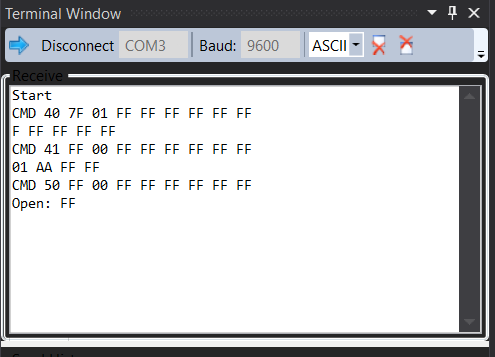
\includegraphics[width=0.5\textwidth]{Figur/SDuartOpen.png}
	\caption{Terminalvindueunder debug af SD driver}
	\label{fig:SDopen}
\end{figure}

På figur \ref{fig:SDopen} ses terminalvinduet for en test, hvor der læses en fil fra SD kortet. Kommandoen står først i Hex efter CMD, hvor 40 er CMD0, og derefter svaret.\\ 
Der forekommer en fejl ved sidste linje, da driveren skal åbne og læse filen. Der fanges programmet i et evigt loop, med ingen respons, hvilket umuliggør implementering i den nuværende form. På \ref{fig:SDprison} ses assembler instruktionen, som driveren fanges i.

\begin{figure}[H]
	\center
	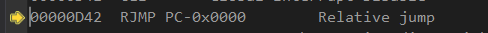
\includegraphics[width=0.5\textwidth]{Figur/SDopenPrison.png}
	\caption{Assembler kodeudsnit ved fejlimplementering}
	\label{fig:SDprison}
\end{figure}
